% 86-29(86쪽) — 한 변의 길이가 9인 정사각형 종이의 네 귀퉁이에서 같은 크기의 정사각형을 잘라 낸 전개도. 스캔 화질이 낮아 TikZ 로 다시 그림.
% 원문에 있는 것만: 회색으로 칠한 남은 부분 · 잘라 낸 네 귀퉁이(흰 정사각형) · 접는 선(점선) · 치수 9 둘(점선 호). 잘라 내는 정사각형의 한 변은 원문에 값이 없으므로 적지 않는다.
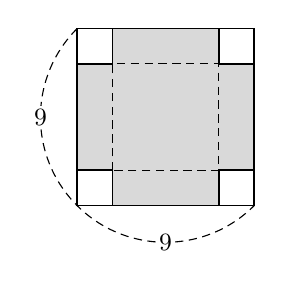
\begin{tikzpicture}[x=0.25cm, y=0.25cm, line width=0.5pt]
  \fill[black!15] (0,0) rectangle (9,9);
  \fill[white] (0,7.2) rectangle (1.8,9);
  \fill[white] (7.2,7.2) rectangle (9,9);
  \fill[white] (0,0) rectangle (1.8,1.8);
  \fill[white] (7.2,0) rectangle (9,1.8);
  \draw[line width=0.6pt] (0,0) rectangle (9,9);
  \draw[line width=0.6pt] (1.8,9) -- (1.8,7.2) -- (0,7.2);
  \draw[line width=0.6pt] (7.2,9) -- (7.2,7.2) -- (9,7.2);
  \draw[line width=0.6pt] (1.8,0) -- (1.8,1.8) -- (0,1.8);
  \draw[line width=0.6pt] (7.2,0) -- (7.2,1.8) -- (9,1.8);
  \draw[densely dashed, line width=0.4pt] (1.8,1.8) rectangle (7.2,7.2);
  \draw[densely dashed, line width=0.4pt] ([shift=(135:6.36)]4.5,4.5) arc (135:315:6.36);
  \node[fill=white, inner sep=1pt, font=\small] at (-1.86,4.5) {$9$};
  \node[fill=white, inner sep=1pt, font=\small] at (4.5,-1.86) {$9$};
\end{tikzpicture}
